% Packages

\documentclass[
	11pt, % Set the default font size, options include: 8pt, 9pt, 10pt, 11pt, 12pt, 14pt, 17pt, 20pt
	%t, % Uncomment to vertically align all slide content to the top of the slide, rather than the default centered
	%aspectratio=169, % Uncomment to set the aspect ratio to a 16:9 ratio which matches the aspect ratio of 1080p and 4K screens and projectors
]{beamer}
\setcounter{tocdepth}{1}
\usepackage{graphicx}
\usepackage[export]{adjustbox}
\graphicspath{{Images/}{./}} % Specifies where to look for included images (trailing slash required)
\usepackage{tikz}
\newenvironment{amatrix}[1]{%
  \left[\begin{array}{@{}*{#1}{c}|c@{}}
}{%
  \end{array}\right]
}

\usepackage{booktabs} % Allows the use of \toprule, \midrule and \bottomrule for better rules in tables
\usepackage{pgfplots}
\usepackage{tikz}
\pgfplotsset{width=6cm, compat=newest, every tick label/.append style={scale=0.5}}
\usepackage{amsmath}
\usepackage{blkarray}% http://ctan.org/pkg/blkarray
\newcommand{\matindex}[1]{\mbox{\scriptsize#1}}% Matrix index

% Theme
\usetheme{Madrid}

% Font
\usefonttheme{serif}
\usepackage{newtxtext,newtxmath}
\usepackage[default]{lato}

% Inner theme
\useinnertheme{circles}

% Information
\title{Matrix}
\author{Kin Hei Wong}
\date{\today}
%%%%%%%%%%%%%%%%%%%%%%%%%%%%%%%%%%%%%%%%%%%%%%%%%%%%%%%%%%
\begin{document}
% Title slide
\begin{frame}
    \titlepage
\end{frame}

% Table of Content
\begin{frame}
    \frametitle{Presentation overview}
    \tableofcontents
\end{frame}
%%%%%%%%%%%%%%%%%%%%%%%%%%%%%%%%%%%%%%%%%%%%%%%%%%%%%%%%%%%
% Body slides

\section{11A: Matrix notation}
\begin{frame}
    \frametitle{11A}
    \begin{center}
        \title{Matrix notation}
        \maketitle
    \end{center}
\end{frame}

\begin{frame}{Matrix}
    A matrix is a rectangular array of numbers. The numbers in the array are called the entries.\\
    \[
        \begin{bmatrix}
        1 & 2 & 3\\
        4 & 5 & 6
    \end{bmatrix}
    \]
    \bigskip
    \begin{block}{Size}
        The size of the matrix is determined by $m$ $\times$ $n$, where $m$ is the row, $n$ is the columns.
    \end{block}
    $\therefore$ the size of the matrix above is 2 $\times$ 3.
\end{frame}

\begin{frame}{Use of matrix?}
    It can be use to store information, as demonstrated below:\\
    \begin{block}{Example}
        Four exporters A, B, C and D sell refrigerators (r), dishwashers (d), microwave ovens (m) and
        televisions (t). The sales in a particular month can be represented by a 4 $\times$ 4 array of numbers.
        This array of numbers is called a matrix.
    \end{block}
    \[
    \begin{blockarray}{ccccc}
        & r & d & m & t & \\
        \begin{block}{c[cccc]}
            A & 120 & 95 & 370 & 250\\
            B & 430 & 380 & 950 & 900\\
            C & 60 & 50 & 150 & 100\\
            D & 200 & 100 & 470 & 50\\
        \end{block}
    \end{blockarray}
    \]
\end{frame}

\begin{frame}[t]
    \frametitle{Example}
    A minibus has four rows of seats, with three seats in each row. If 0 indicates that a seat is
    vacant and 1 indicates that a seat is occupied, write down a matrix to represent:\\
    \begin{enumerate}[(a)]
        \item the 1st and 3rd rows are occupied, but the 2nd and 4th rows are vacant
        \item only the seat at the front-left corner of the minibus is occupied.
    \end{enumerate}
\end{frame}

\begin{frame}[t]
    \frametitle{Example}
    There are four clubs in a local football league:\\
    \begin{enumerate}
        \item Club A has 2 senior teams and 3 junior teams.
        \item Club B has 2 senior teams and 4 junior teams.
        \item Club C has 1 senior team and 2 junior teams.
        \item Club D has 3 senior teams and 3 junior teams.
    \end{enumerate}
    Represent this information in a matrix.
\end{frame}

\begin{frame}{Entries and equality}
    \begin{block}{}
        If A is a matrix, then $a_{ij}$ will be used to denote the entry that occurs in row i and column j
    of A.
    \end{block}
    Thus a 3 $\times$ 4 matrix may be written as\\
    \[A = 
    \begin{bmatrix}
        a_{11} & a_{12} & a_{13} & a_{14}\\
        a_{21} & a_{22} & a_{23} & a_{24}\\
        a_{31} & a_{32} & a_{33} & a_{34}\\
    \end{bmatrix}
    \]
\end{frame}
\begin{frame}{Exercise: 11A}
\end{frame}
%%%%%%%%%%%%%%%%%%%%%%%%%%%%%%%%%%%%%%%%%%%%%%%%%%%%%%%%%%%%%%%%%%%%%%%%%%%%%%%%%%%%%%%%%%%%%
\section{11B: Addition, subtraction and multiplication by a real number}
\begin{frame}
    \frametitle{11B}
    \begin{center}
        \title{Addition, subtraction and multiplication by a real number}
        \maketitle
    \end{center}
\end{frame}

\begin{frame}{Addition and subtraction}
    In addition and subtraction, we just add it individually according to the position. \alert{HOWEVER}, you must make sure
    that they are in the same size!\\
    \bigskip
    \[
    \begin{bmatrix}
        a_{11} & a_{12} \\
        a_{21} & a_{22} \\
        a_{31} & a_{32}
    \end{bmatrix}
    +
    \begin{bmatrix}
        b_{11} & b_{12} \\
        b_{21} & b_{22} \\
        b_{31} & b_{32}
    \end{bmatrix}
    =
    \begin{bmatrix}
        a_{11} + b_{11} & a_{12} + b_{12}\\
        a_{21} + b_{21} & a_{22} + b_{22}\\
        a_{31} + b_{31} & a_{32} + b_{32}
    \end{bmatrix}
    \]
\end{frame}

\begin{frame}{Multiplication of a matrix by a real number}
    If A is any matrix and k is a real number, then the product kA is the matrix obtained by
    multiplying each entry of A by k.\\
    \[
    3
    \begin{bmatrix}
        2 & -2\\
        0 & 1
    \end{bmatrix}
    =
    \begin{bmatrix}
        6 & -6\\
        0 & 3
    \end{bmatrix}
    \]
\end{frame}

\begin{frame}{Zero matrix}
    The m $\times$ n matrix with all entries equal to zero is called the zero matrix, and will be
    denoted by \textbf{O}.\\
    \begin{block}{}
        For any m $\times$ n matrix $A$ and the m $\times$ n zero matrix \textbf{O}, we have\\
    $A + \textbf{O} = A$ and $A + (-A) = \textbf{O}$
    \end{block}
\end{frame}

\begin{frame}[t]
    \frametitle{Example}
    Let 
    \[
        X = 
    \begin{bmatrix}
        2\\
        4
    \end{bmatrix}
    , Y =
    \begin{bmatrix}
        3\\
        6
    \end{bmatrix}
    \text{, A =} 
    \begin{bmatrix}
        2 & 0\\
        -1 & 2
    \end{bmatrix}
    \text{and B = }
    \begin{bmatrix}
        5 & 0\\
        -2 & 4
    \end{bmatrix}
    .
    \]
    Find X + Y, 2X, 4Y + X, X - Y, -3A and 3A + B.
\end{frame}

\begin{frame}
\end{frame}
\begin{frame}{Exercise: 11B}
\end{frame}
%%%%%%%%%%%%%%%%%%%%%%%%%%%%%%%%%%%%%%%%%%%%%%%%%%%%%%%%%%%%%%%%%%%%
\section{11C: Multiplication of matrices}
\begin{frame}
    \frametitle{11C}
    \begin{center}
        \title{Multiplication of matrices}
        \maketitle
    \end{center}
\end{frame}

\begin{frame}{Multiplication by matrices is less straightforward!}
    \begin{block}{Multiplication by matrices}
        If A is an m $\times$ n matrix and B is an n $\times$ r matrix, then the product AB is the m $\times$ r matrix
        whose entries are determined as follows:
        To find the entry in row i and column j of AB, single out row i in matrix A and
        column j in matrix B. Multiply the corresponding entries from the row and column
        and then add up the resulting products.
    \end{block}
\end{frame}

\begin{frame}
    \begin{alertblock}{TOO LONG TO UNDERSTAND}
        Just keep in mind of these things:
        \begin{enumerate}
            \item To find first row and first column of the result, multiply the number of first row, first column individually and add together
            \item To find first row and second column of the result, multiply the number of first row, second column individually and add together
            \item I believe, you see the pattern: but I will demonstrate later
            \item If the product AB is only defined iff(if and only if) \alert{number of columns of A = number of rows of B}
        \end{enumerate}
    \end{alertblock}
\end{frame}

\begin{block}{Demonstration}
    Note: it is always row $\times$ column.\\
    Let 
    \[
        \text{A = }
        \begin{bmatrix}
            1 & 3\\
            4 & 2
        \end{bmatrix}
        \text{and B = }
        \begin{bmatrix}
            5 & 1\\
            6 & 3
        \end{bmatrix}
    \]
    Then 
    \[
        AB = 
        \begin{bmatrix}
            1 \times 5 + 3 \times 6 & 1 \times 1 + 3 \times 3\\
            4 \times 5 + 2 \times 6 & 4 \times 1 + 2 \times 3
        \end{bmatrix}
        =
        \begin{bmatrix}
            23 & 10\\
            32 & 10
        \end{bmatrix}
    \]
    Then
    \[
        BA = 
        \begin{bmatrix}
            1 \times 5 + 1 \times 4 & 5 \times 3 + 1 \times 2\\
            6 \times 1 + 3 \times 4 & 6 \times 3 + 3 \times 2
        \end{bmatrix}
        =
        \begin{bmatrix}
            9 & 17\\
            18 & 24
        \end{bmatrix}
    \]
\end{block}
\begin{block}{Quickfire question}
    What do you notice between AB and BA?
\end{block}
\begin{frame}{Exercise: 11C}
\end{frame}
%%%%%%%%%%%%%%%%%%%%%%%%%%%%%%%%%%%%%%%%%%%%%%%%%%%%%%%%%%%%%%%%%%%%%%%%%%%%%%%%%%%%%%%%%%%%%%%%%%%%%%%%%%%%%%%%%%%%%%%%%%%%%%%%%%%%
\section{11D: Identities, inverses and determinants for 2 $\times$ 2 matrices}
\begin{frame}
    \frametitle{11D}
    \begin{center}
        \title{Identities, inverses and determinants for 2 $\times$ 2 matrices}
        \maketitle
    \end{center}
\end{frame}

\begin{frame}{What is identity matrix?}
    Identiy matrix of n $\times$ n is\\
    \[
    \begin{bmatrix}
        1 & 0 &\ldots & 0\\
        0 & 1 &\ldots & 0\\
        \vdots&\vdots & \ddots & \vdots\\
        0 & 0 & \ldots& 1
    \end{bmatrix}
    \]
    This assumes that n in finite! Then, if we assume n = 2?\\
    \[
    \begin{bmatrix}
        1 & 0\\
        0 & 1
    \end{bmatrix}
    \]
    \begin{block}{}
        Try multiplying identity matrix with any matrix, what do you notice? What can we conclude?
    \end{block}
\end{frame}

\begin{frame}{Identity matrix property!}
    Let A be a matrix of n $\times$ n (or we call it square matrix). Then, AI = A = IA. This also means the A is invertible.\\
    \bigskip
    \begin{block}{Invertible matrix}
        For an invertible matrix A, we have\\
        \[
            AA^{-1} = I = A^{-1}A
        \]
    \end{block}
    We will start to learn more the next slide.
\end{frame}

\begin{frame}{Inverse matrix}
    From any non-zero real number $x$, there is a real number $x^{-1}$, which has the result of $xx^{-1} = 1.$\\
    It is the same in matrix!
    \begin{block}{Example}
        Consider 
        \[
            A =
            \begin{bmatrix}
                2 & 3\\
                1 & 4
            \end{bmatrix}
            B = 
            \begin{bmatrix}
                x & y\\
                u & v
            \end{bmatrix}
        \]
        and AB = I. Solve matrix B.
    \end{block}
\end{frame}
\begin{frame}{The usual way}
\end{frame}

\begin{frame}[t]
    \frametitle{General 2 $\times$ 2 matrix}
    Let
    \[
        A = 
        \begin{bmatrix}
            a & b\\
            c & d
        \end{bmatrix}
        \text{,} B = 
        \begin{bmatrix}
            x & y\\
            u & v
        \end{bmatrix}
    \]
    and AB = I implies\\
    \[
        \begin{bmatrix}
            a & b\\
            c & d
        \end{bmatrix}
        \begin{bmatrix}
            x & y\\
            u & v
        \end{bmatrix}
        =
        \begin{bmatrix}
            1 & 0\\
            0 & 1
        \end{bmatrix}
    \]
\end{frame}
\begin{frame}[b]
    \frametitle{Here comes determinant!}
    \begin{block}{Inverse of 2 $\times$ 2 matrix}
        If 
        \[
            A =
            \begin{bmatrix}
                a & b\\
                c & d
            \end{bmatrix}
        \], then the inverse of A is given by\\
        \[
            A^{-1} = \dfrac{1}{ad-bc}
            \begin{bmatrix}
                d & -b\\
                -c & a
            \end{bmatrix}
            \quad (\text{provided } ad-bc \neq 0)
        \]
    \end{block}
\end{frame}

\begin{frame}{Determinant}
    If 
        \[
            A =
            \begin{bmatrix}
                a & b\\
                c & d
            \end{bmatrix}
        \]
        then det(A) = $ad - bc$.\\
        Note: 2 $\times$ 2 matrix A has an inverse only if det(A) $\neq$ 0.
\end{frame}

\begin{frame}{Application of inverse matrix}
    A common way of sending an encrypted message is to assign an integer value to each letter of the alphabet and send the message as a string of integers.\\
    E.g. The message: (SEND MONEY) can be sent as 5,8,10,21,7,2,10,8,3.\\
    A more secure way is to use matrix multiplication and matrix inverses! This is because we can use the inverse matrix to decrypting the message\\
    Slide adapted from UoM: MAST10007 Linear Algebra Lecture Notes 2021
\end{frame}

\begin{frame}{Exercise: 11D}
\end{frame}
%%%%%%%%%%%%%%%%%%%%%%%%%%%%%%%%%%%%%%%%%%%%%%%%%%%%%%%%%%%%%5
\section{11E: Solution of simultaneous equation}
\begin{frame}
    \frametitle{11D}
    \begin{center}
        \title{Identities, inverses and determinants for 2 $\times$ 2 matrices}
        \maketitle
    \end{center}
\end{frame}

\begin{frame}{Simultaneous in matrices}
    We can represent the simultaneous of:\\
    $3x-2y=5$\\
    $5x-3y=9$\\
    into
    \[
        \begin{bmatrix}
            3 & -2\\
            5 & -3
        \end{bmatrix}
        \begin{bmatrix}
            x\\
            y
        \end{bmatrix}
        =
        \begin{bmatrix}
            5\\
            9
        \end{bmatrix}
    \]
\end{frame}

\begin{frame}[t]
    \frametitle{Solving simultaneous in matrices}
    Note: If determinant of the matrix is 0, then there is no UNIQUE solution.
    \[
        \text{Let A = }
        \begin{bmatrix}
            3 & -2\\
            5 & -3
        \end{bmatrix}
        \therefore, \text{A}^{-1} =
        \begin{bmatrix}
            -3 & 2\\
            -5 & -3
        \end{bmatrix}
    \]
\end{frame}

\begin{frame}[t]
    \frametitle{Example}
    \[
        \text{Let A =}
        \begin{bmatrix}
            2 & -1\\
            1 & 2
        \end{bmatrix},
        \text{K =}
        \begin{bmatrix}
            -1\\
            2
        \end{bmatrix}
        . \text{Solve the system AX = K, where X =}
        \begin{bmatrix}
            x\\
            y
        \end{bmatrix}
    \]
\end{frame}

\begin{frame}[t]
    \frametitle{Example}
    Solve the following simultaneous equations:\\
    $3x - 2y = 6$\\
    $7x + 4y = 7$
\end{frame}
\begin{frame}{Exercise: 11E}
\end{frame}
%%%%%%%%%%%%%%%%%%%%%%%%%%%%%%%%%%%%%%%%%%%%%%%%%%%%%%%%%%%%%%%%%%%%%%%%%%%%%%%%%%%%%%%%%%%%
\section{11F: Inverse and determinants for $n \times n$ matrices}
\begin{frame}
    \frametitle{11F}
    \begin{center}
        \title{Inverse and determinants for $n \times n$ matrices}
        \maketitle
    \end{center}
\end{frame}

\begin{frame}[t]
    \frametitle{Finding inverse of $3 \times 3$}
    Without using a calculator, find the inverse of matrix
    \[
        \text{A =}
        \begin{bmatrix}
            1 & -3 & 2\\
            -3 & 3 & -1\\
            2 & -1 & 0
        \end{bmatrix}
    \]
    Note: There is more efficient method known as Gaussian's elimination.
\end{frame}
\begin{frame}    
\end{frame}

\begin{frame}{Finding determinant}
    We can use the method of Cofactor expansion:
    \begin{block}{Definition}
        Let A be a square matrix. The \alert{$(i, j)$-cofactor} of A denoted by $C_{ij}$, is the number given by\\
        $C_{ij} = (-1)^{i+j}det(A(i,j))$\\
        where $A(i,j)$ is the matrix obtained from A by deleting the ith row and jth column.
    \end{block}
    How do we remember the sign of cofactor?\\
    \[
    \begin{bmatrix}
        + & - & + & \ldots\\
        - & + & - & \ldots\\
        + & - & + & \ldots\\
        \vdots & \vdots & \vdots & \ddots
    \end{bmatrix}
    \]
\end{frame}

\begin{frame}[t]
    \frametitle{Example}
    \[
        \text{Let A = }
        \begin{bmatrix}
            a_{11} & a_{12} & a_{13}\\
            a_{21} & a_{22} & a_{23}\\
            a_{31} & a_{32} & a_{33}\\
        \end{bmatrix}
    \]
\end{frame}

\begin{frame}    
\end{frame}
\begin{frame}[t]
    \frametitle{Example}
    \[
        \text{Let A = }
        \begin{bmatrix}
            3 & 2 & 0\\
            3 & 4 & 1\\
            2 & 1 & 2\\
        \end{bmatrix}
    \]
\end{frame}
\begin{frame}
\end{frame}
\begin{frame}{Exercise: 11F}
\end{frame}
%%%%%%%%%%%%%%%%%%%%%%%%%%%%%%%%%%%%%%%%%%%%%%%%%%%%%%%%%%%%%%%%%%%%%%%%%%%%%%%%%%%%%%%%%%%%%%%%%%%%%
\section{11G: Simultaneous linear equations with more than two variables}
\begin{frame}
    \frametitle{11G}
    \begin{center}
        \title{Simultaneous linear equations with more than two variables}
        \maketitle
    \end{center}
\end{frame}

\begin{frame}[t]
    \frametitle{Linear equations in three variables}
    Consider the general system of three linear equations in three variables:
    $a_1x + b_1y+ c_1z = d_1$\\
    $a_2x + b_2y+ c_2z = d_2$\\
    $a_3x + b_3y+ c_3z = d_3$
    \[
        \begin{bmatrix}
            a_1 & b_1 & c_1\\
            a_2 & b_2 & c_2\\
            a_3 & b_3 & c_3
        \end{bmatrix}
        \begin{bmatrix}
            x\\
            y\\
            z
        \end{bmatrix}
        =
        \begin{bmatrix}
            d_1\\
            d_2\\
            d_3
        \end{bmatrix}
    \]
    \[
        \text{Let A =} 
        \begin{bmatrix}
            a_1 & b_1 & c_1\\
            a_2 & b_2 & c_2\\
            a_3 & b_3 & c_3
        \end{bmatrix}
        \text{,X =}
        \begin{bmatrix}
            x\\
            y\\
            z
        \end{bmatrix}
        \text{and B =}
        \begin{bmatrix}
            d_1\\
            d_2\\
            d_3
        \end{bmatrix}
    \]    
    Then, AX = B
\end{frame}

\begin{frame}[t]
    \frametitle{Example}
    Use matrix method to solve the following system of three equations in three variables:\\
    $2x + y + z = -1$\\
    $3y + 4z = -7$\\
    $6x + z = 8$
\end{frame}
\begin{frame}[b]
    Note: Possible cases for a system of three linear equations in three variables:
    \begin{enumerate}
        \item A unique solution
        \item no solution
        \item infinitely many solutions
    \end{enumerate}    
\end{frame}

\begin{frame}{Exercise: 11G}
\end{frame}
%%%%%%%%%%%%%%%%%%%%%%%%%%%%%%%%%%%%%%%%%%%%%%%%%%%%%%%%%%%%%%%%%%%%%%%%%%%%%%%%%%%%%%%%%%%%%%%%%%%%%
\section{Extra: Gaussian elimination}
\begin{frame}
    \frametitle{Extra}
    \begin{center}
        \title{Gaussian elimination}
        \maketitle
    \end{center}
\end{frame}

\begin{frame}
    \frametitle{How to do Gaussian elimination?}
    Gaussian elimination is a systematic way to reduce a matrix to row-echelon form using row operations.
    \begin{block}{Gaussian elimination}
        \begin{enumerate}
            \item Interchange rows if necessary, to bring a non-zero number to the top of the first column with a non-zero entry.
            \item Add suitable multiples of the top row to lower rows so that all entries below the leading entry are zero. (Multiplying a row
            by a constant is also allowed and is often useful.)
            \item Start again in Step 1 applied to the matrix without the first row.
        \end{enumerate}
    \end{block}
    \begin{block}{Example of row-echelon}
        \[
        \begin{bmatrix}
            1 & -2 & 3 & 4 & 5
        \end{bmatrix}
        \]
        \[
        \begin{amatrix}{2}
            1 & 2 & 3\\
            a & b & c
        \end{amatrix}
        \]
    \end{block}
\end{frame}

\begin{frame}{How is this useful?}
    This is the most efficient way to solve for:
    \begin{block}{}
        \begin{enumerate}
            \item Systematic solver
            \item Finding inverse matrix
        \end{enumerate}
    \end{block}
\end{frame}
\begin{frame}[t]
    \frametitle{Example}
    Make the matrix into row-echelon form
    \[
        \begin{bmatrix}
            2 & 5 & 3\\
            3 & 6 & 9\\
            4 & 8 & 1
        \end{bmatrix}
    \]
\end{frame}

\begin{frame}[t]
    \frametitle{Example}
    Solve the following system using Gaussian elimination:\\
    $x - 3y + 2z = 11$\\
    $2x - 3y - 2z = 13$\\
    $4x - 2y + 5z = 31$
\end{frame}
\begin{frame}
\end{frame}

\begin{frame}[t]
    \frametitle{Example - Inverse matrix}
    Find the inverse of 
    \[
        \text{A = }
        \begin{bmatrix}
            1 & 2 & 1\\
            -1 & -1 & 1\\
            0 & 1 & 3
        \end{bmatrix}
    \]
    Solution:\\
    Form the augmented matrix $[A|I_3]$ and perform row operations so that A is in reduced row-echelon form.
\end{frame}
\begin{frame}    
\end{frame}

\begin{frame}{This comes to the end of Matrix...}
    Want to learn more? Explore around Linear Algebra or here is a free text website below\\
    \url{https://hefferon.net/}\\
    \begin{center}
        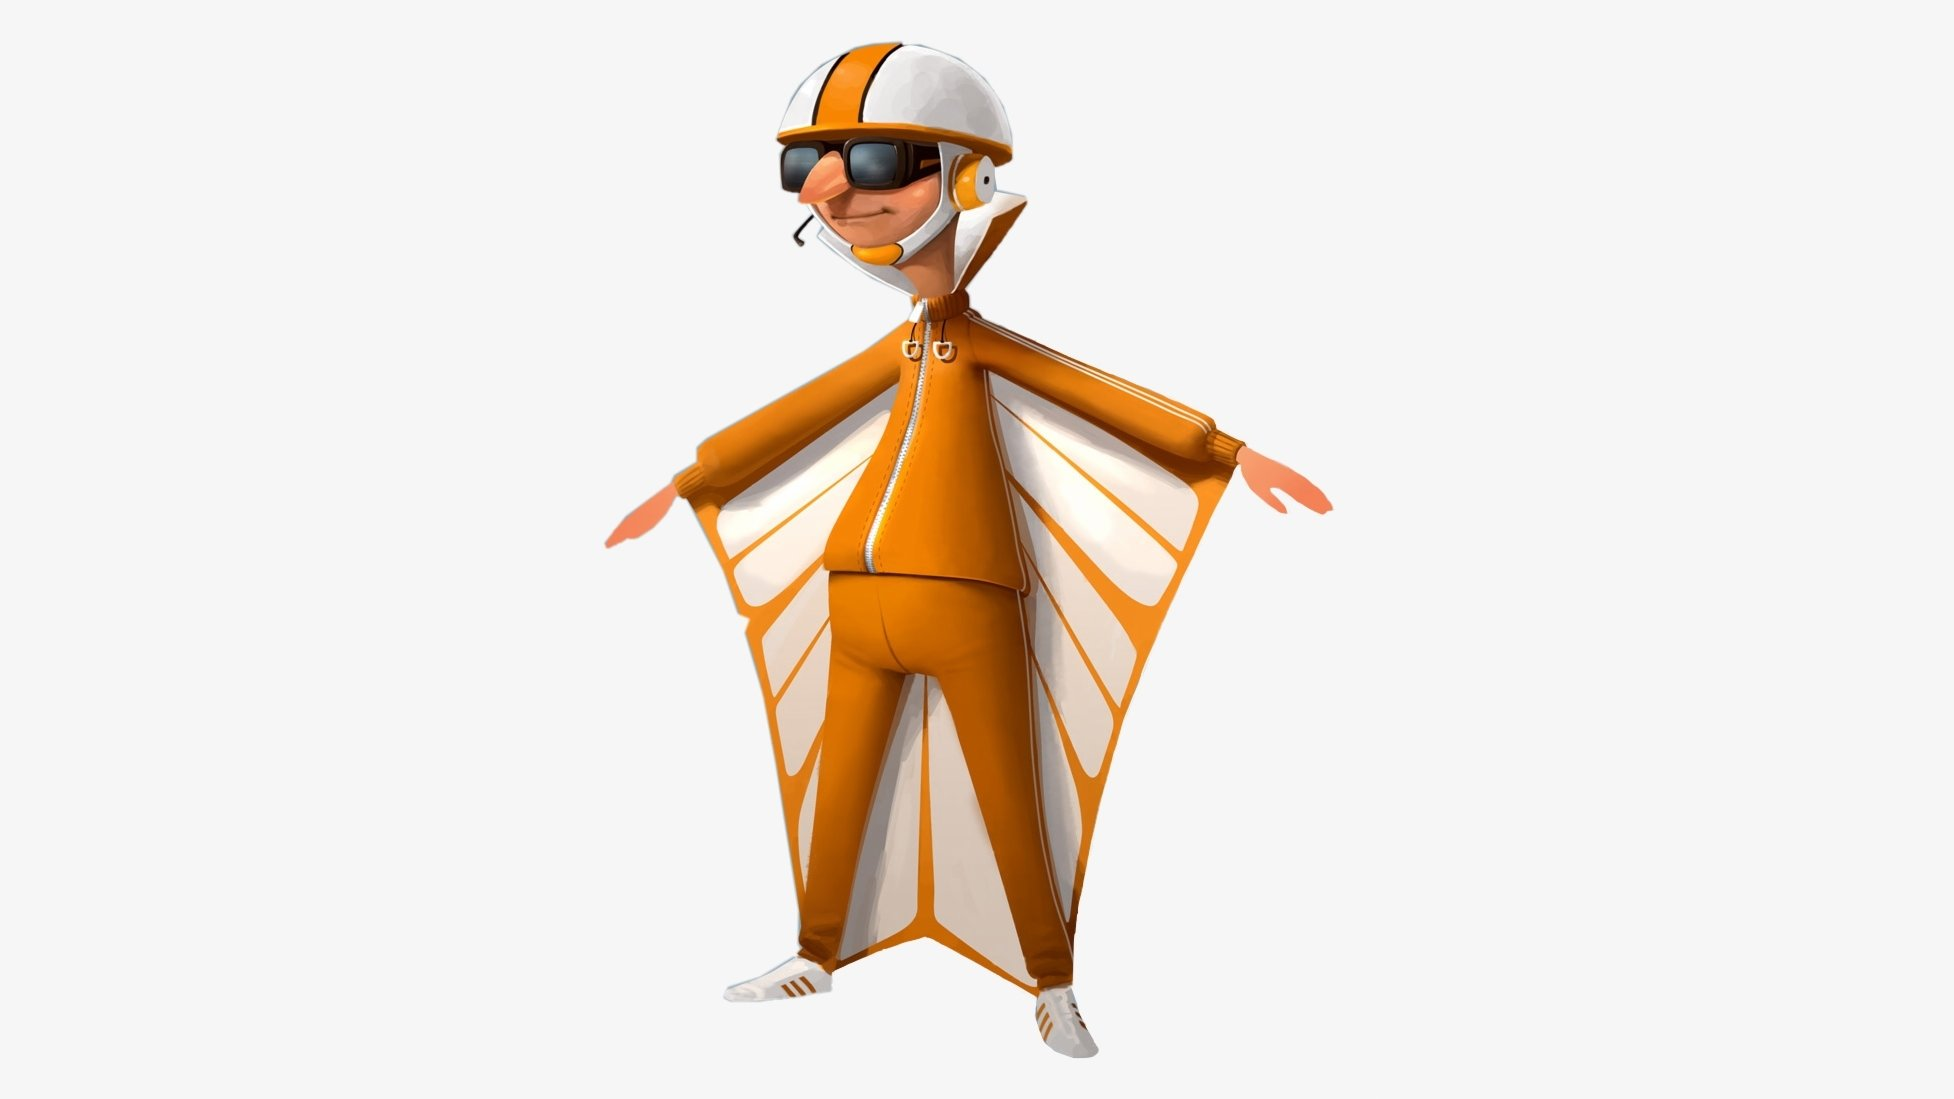
\includegraphics[width=0.5\textwidth]{Vector.jpg}
    \end{center}
\end{frame}
\end{document}